% =====================================================================
%  draft.tex  —  Atualização do VessShape paper (4 datasets, novos modelos)
%  Blocos rotulados por destino em main.tex. NÃO é para substituir main.tex;
%  é material para o autor revisar e transplantar bloco a bloco.
%
%  Este arquivo é autocompilável (pdflatex draft.tex) graças ao preâmbulo
%  mínimo abaixo. As referências \cite/\ref aparecem como ?? aqui — normal,
%  pois só resolvem dentro de main.tex. O conteúdo entre os marcadores
%  "% #####" é o que deve ser transplantado para main.tex.
% =====================================================================
\pdfminorversion=7
\pdfobjcompresslevel=0
\documentclass[twocolumn]{article}
\usepackage[a4paper,margin=1.6cm]{geometry}
\usepackage{graphicx,booktabs,multirow,tabularx,amsmath,amssymb,url}
\graphicspath{{figures/}}
\begin{document}


% #####################################################################
% # 0. BIBLIOGRAFIA — acrescentar a references.bib
% #####################################################################
% --- DCA1 (fornecido pelo autor) ---
% @article{Cervantes2019,
%   title   = {Automatic segmentation of coronary arteries in {X-ray} angiograms using multiscale analysis and artificial neural networks},
%   author  = {Cervantes-Sanchez, Fernando and Cruz-Aceves, Ivan and Hernandez-Aguirre, Arturo and Hernandez-Gonzalez, Martha A. and Solorio-Meza, Sergio E.},
%   journal = {Applied Sciences}, volume = {9}, number = {24}, pages = {5507}, year = {2019},
%   doi     = {10.3390/app9245507} }
%
% --- OCTA-500 / OCTA2D (fornecido pelo autor) ---
% @article{Li2020_OCTA500,
%   title   = {{OCTA-500}: A retinal dataset for optical coherence tomography angiography study},
%   author  = {Li, Mingchao and Huang, Kun and Xu, Qiuzhuo and Yang, Jiadong and Zhang, Yuhan and Ji, Zexuan and Xie, Keren and Yuan, Songtao and Liu, Qinghuai and Chen, Qiang},
%   journal = {IEEE Transactions on Medical Imaging}, year = {2024},
%   doi     = {10.1109/TMI.2024.3354408} }
%
% --- MedSAM / LiteMedSAM  % CONFIRMAR (não fornecido; provável entrada abaixo) ---
% @article{ma2024medsam,
%   title   = {Segment anything in medical images},
%   author  = {Ma, Jun and He, Yuting and Li, Feifei and Han, Lin and You, Chenyu and Wang, Bo},
%   journal = {Nature Communications}, volume = {15}, number = {1}, pages = {654}, year = {2024},
%   doi     = {10.1038/s41467-024-44824-z} }


% #####################################################################
% # 1. ABSTRACT  —  substitui o parágrafo do abstract em main.tex (l.121)
% #####################################################################
% >>> DESTINO: \begin{abstract} ... \end{abstract}
%
% (Edição mínima: troca "two real-world datasets" por quatro datasets em três
%  modalidades e cita os novos baselines. Restante do abstract preservado.)

Semantic segmentation of blood vessels is an important task in medical image analysis, but its progress is often hindered by the scarcity of large annotated datasets and the poor generalization of models across different imaging modalities. A key aspect is the tendency of Convolutional Neural Networks (CNNs) to learn texture-based features, which limits their performance when applied to new domains with different visual characteristics. We hypothesize that leveraging geometric priors of vessel shapes, such as their tubular and branching nature, can lead to more robust and data-efficient models. To investigate this, we introduce VessShape, a methodology for generating large-scale 2D synthetic datasets designed to instill a shape bias in segmentation models. VessShape images contain procedurally generated tubular geometries combined with a wide variety of foreground and background textures, encouraging models to learn shape cues rather than textures. We demonstrate that a model pre-trained on VessShape images achieves strong few-shot segmentation performance on four real-world datasets spanning three imaging modalities---retinal fundus photography (DRIVE), retinal OCT angiography (OCTA2D), X-ray coronary angiography (DCA1), and fluorescence microscopy of the cortex (VessMAP)---requiring only a few samples for fine-tuning. Compared against standard ImageNet-pretrained U-Nets and a fine-tuned medical foundation model (LiteMedSAM), the VessShape-pretrained model is markedly stronger in the low-data regime and is the only approach that transfers effectively without any target-specific training. Our results indicate that pre-training with a strong shape bias is an effective strategy to overcome data scarcity and improve model generalization in blood vessel segmentation.


% #####################################################################
% # 2. FIGURA — VessShape generation pipeline
% #    DESTINO: Methodology › The VessShape Generator (após a Fig. f:vessshape_sample, ~l.222)
% #####################################################################
\begin{figure*}[tbp]
    \centering
    \includegraphics[width=\textwidth]{figures/vessshape_generation.pdf}
    \caption{Overview of the VessShape generation pipeline. \textbf{Curve generation} (top row): two endpoints are sampled in the image domain; a set of intermediate control points is added along the connecting line and perturbed to introduce tortuosity; a B\'ezier curve is fitted to these points, rasterized into a 1-pixel-thick polyline, and finally dilated with a disk-shaped structuring element of radius $r_0$ to assign a tubular thickness, producing the binary mask $M$. \textbf{Texturing} (bottom row): a foreground (curve) texture and a background texture are drawn from two different ImageNet classes; an alpha matte is obtained by smoothing $M$ with a Gaussian filter of standard deviation $\sigma$, and the textures are blended following Eq.~\ref{eq:compose} to yield the final VessShape image. The rightmost panel shows the result without Gaussian smoothing ($\sigma \to 0$), which produces hard vessel boundaries.}
    \label{f:vessshape_generation}
\end{figure*}


% #####################################################################
% # 3. FIGURA — Training / progressive-sampling protocol
% #    DESTINO: Methodology › Fine-tuning (após a descrição do protocolo, ~l.308)
% #####################################################################
\begin{figure*}[tbp]
    \centering
    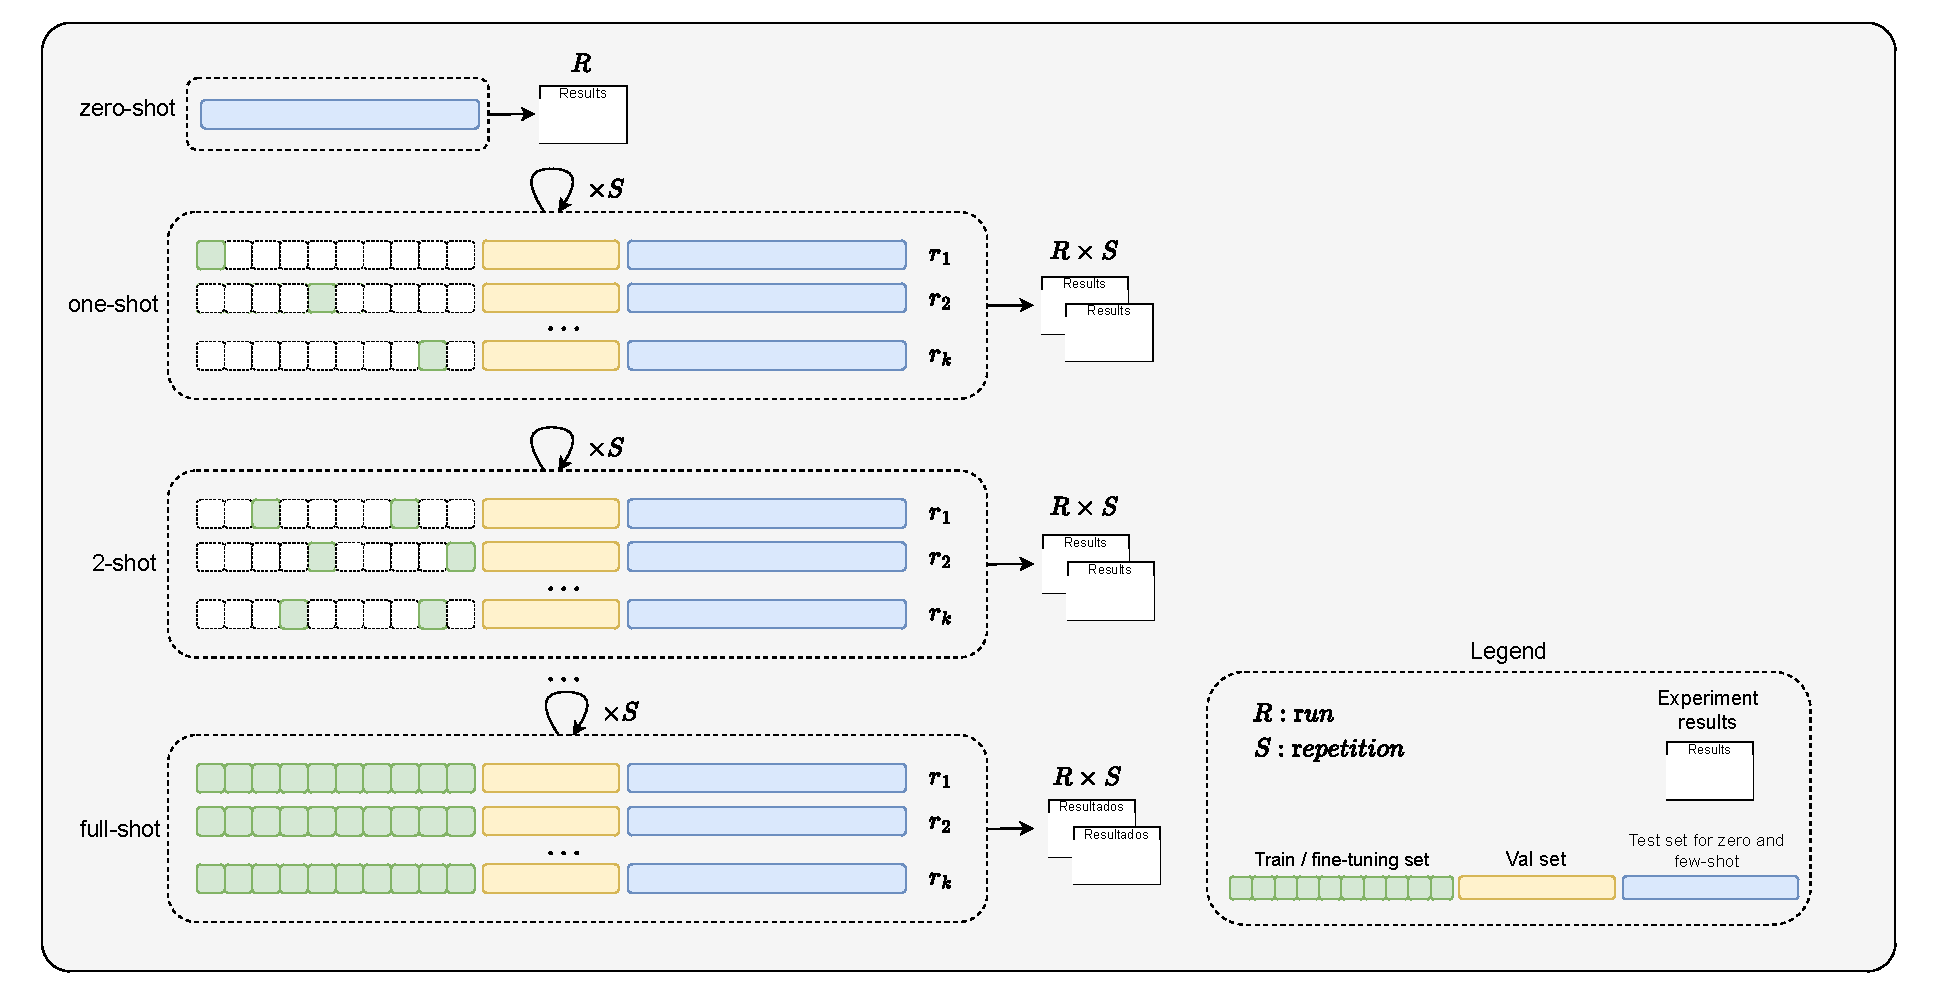
\includegraphics[width=\textwidth]{figures/training_protocol.pdf}
    \caption{Progressive-sampling protocol used for both fine-tuning (VSUNet, IN-UNet, LiteMedSAM-FT) and training from scratch (U-Net). For each sample size $n$ (zero-shot, one-shot, two-shot, \ldots, full-shot), the target training pool (green) is sampled $R$ times without replacement, and each sampled subset is used to train the model $S$ times; validation (yellow) and test (blue) sets are fixed. The zero-shot regime ($n{=}0$) evaluates the pre-trained model directly on the test set, with no target-specific training. This yields $R\times S$ result sets per $n$, allowing the variance to be decomposed into image-combination and optimization components.}
    \label{f:training_protocol}
\end{figure*}


% #####################################################################
% # 4. FIGURAS DE RESULTADOS (Results section)
% #####################################################################

% ---- 4a. Few-shot line charts (SUBSTITUI results_charts.pdf, ~l.367) ----
% NOTA: confirmar a ordem dos painéis no PDF final. Pela inspeção visual:
%       (a) VessMAP, (b) DRIVE, (c) OCTA2D, (d) DCA1.
\begin{figure*}[tbp]
    \centering
    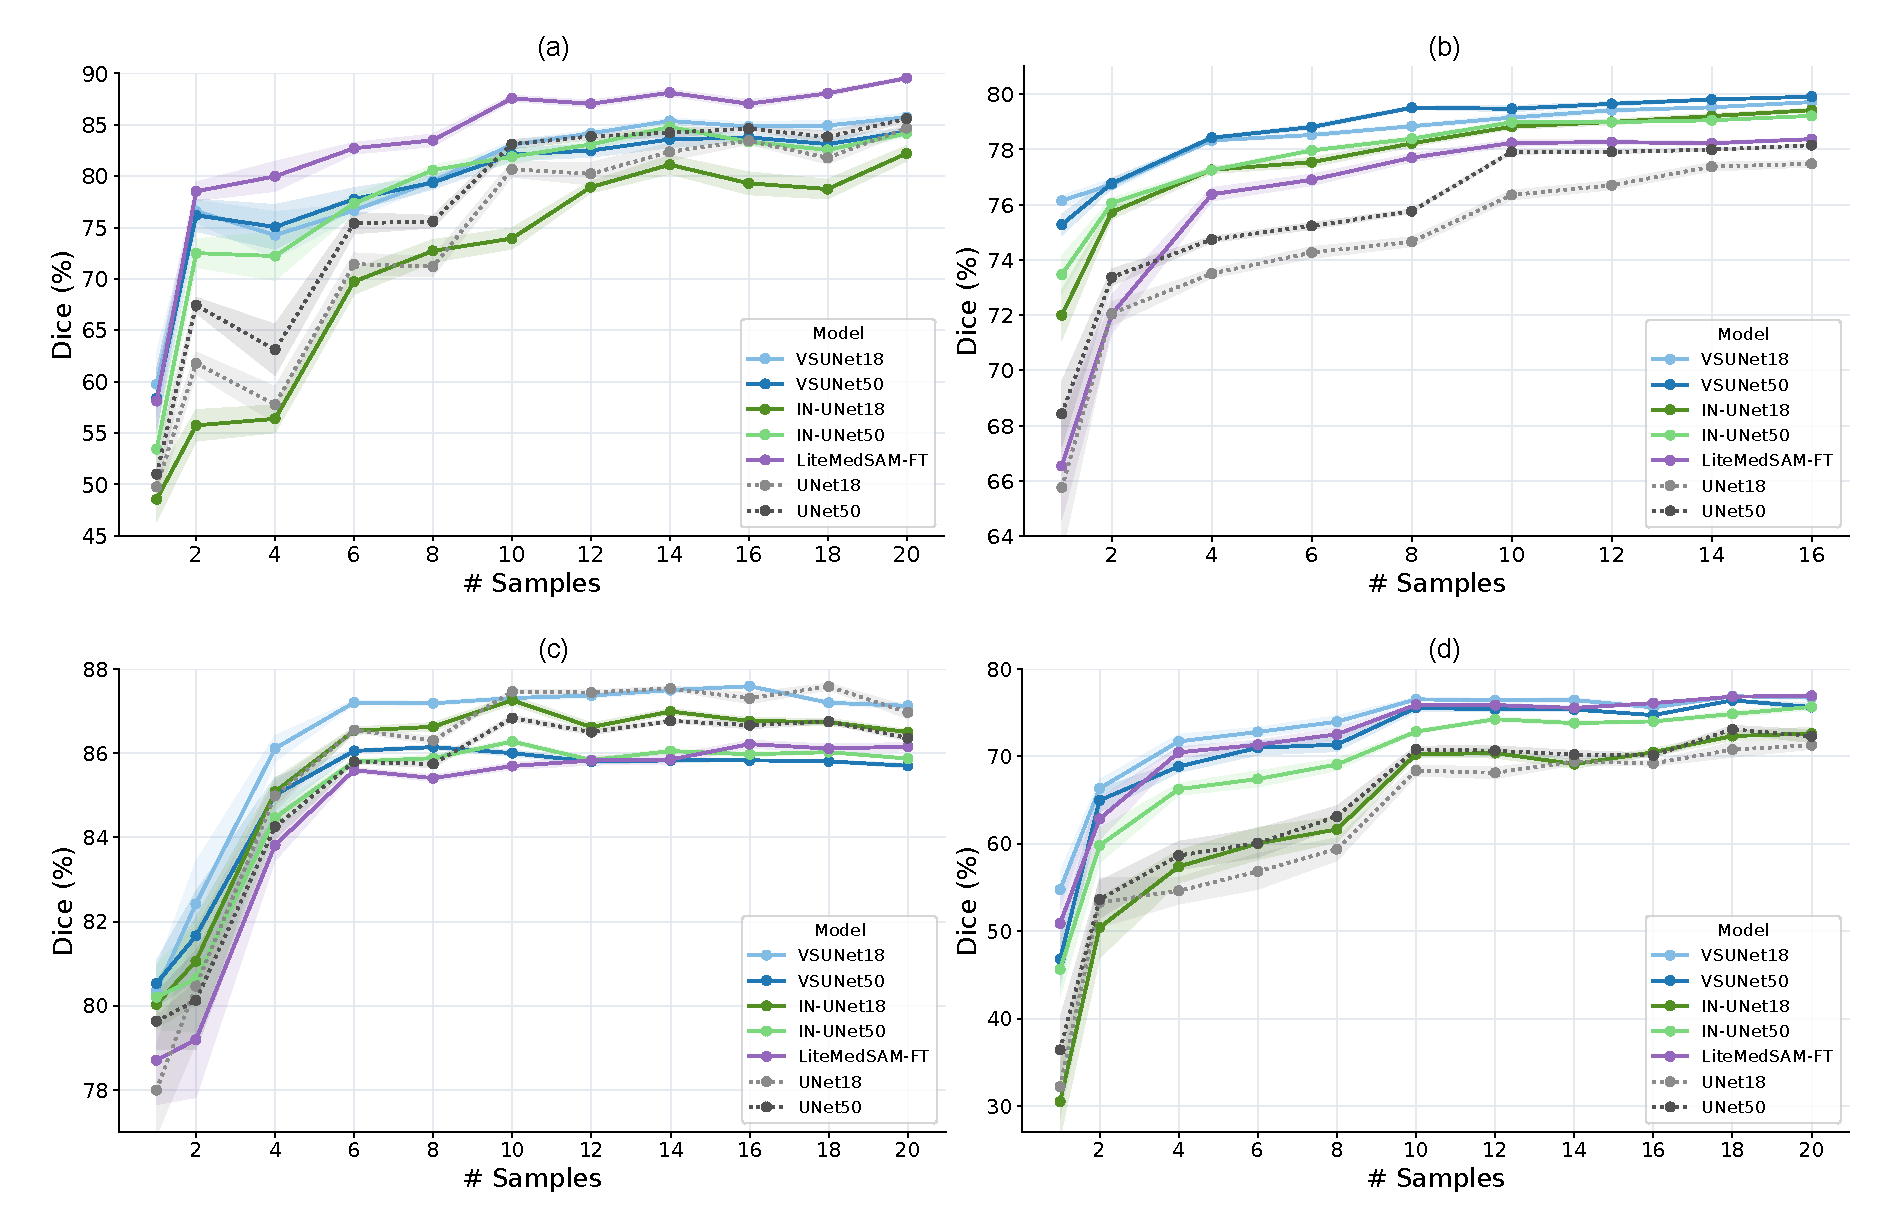
\includegraphics[width=\textwidth]{figures/dice_few_shot_analysis_line_chart.pdf}
    \caption{Few-shot Dice performance as a function of the number of annotated training samples $n$ for (a) VessMAP, (b) DRIVE, (c) OCTA2D and (d) DCA1. Each curve is the mean Dice over $R{=}5$ runs and $S{=}3$ repetitions; shaded areas denote the standard deviation across runs. Seven models are compared: the VessShape-pretrained VSUNet18/50, the ImageNet-pretrained IN-UNet18/50, the fine-tuned LiteMedSAM-FT, and the from-scratch UNet18/50 (dotted). The pre-trained VSUNet variants rise faster and dominate the low-sample regime, while all models tend to converge as $n$ grows.}
    \label{f:results_charts}
\end{figure*}

% ---- 4b. Zero-/one-shot bar charts (nova, Results) ----
\begin{figure*}[tbp]
    \centering
    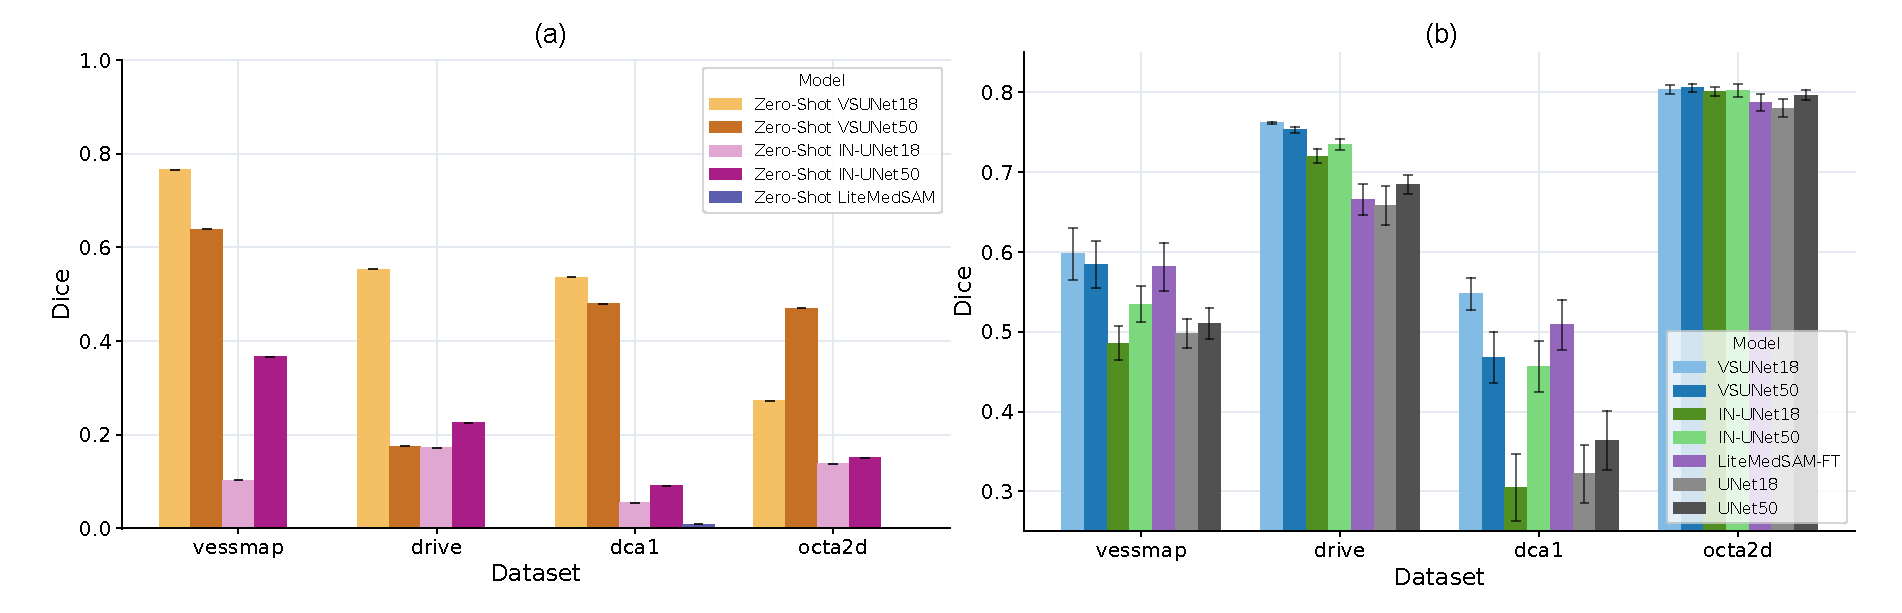
\includegraphics[width=\textwidth]{figures/dice_zero_one_shot_analysis_bar_chart.pdf}
    \caption{Per-dataset Dice in the extreme low-data regimes. (a) Zero-shot Dice ($n{=}0$) for the five variants that admit direct inference: the VessShape-pretrained VSUNet18/50, the ImageNet-pretrained IN-UNet18/50, and LiteMedSAM. Only the VSUNet variants transfer, whereas ImageNet- and MedSAM-initialized models collapse to near-zero Dice. (b) One-shot Dice ($n{=}1$) for all seven models; error bars show the standard deviation across runs. A single labeled example already lets every model produce meaningful segmentations, with the VSUNet variants generally on top.}
    \label{f:bar_zero_one}
\end{figure*}

% ---- 4c. Significance heatmaps (nova, Results) ----
\begin{figure*}[tbp]
    \centering
    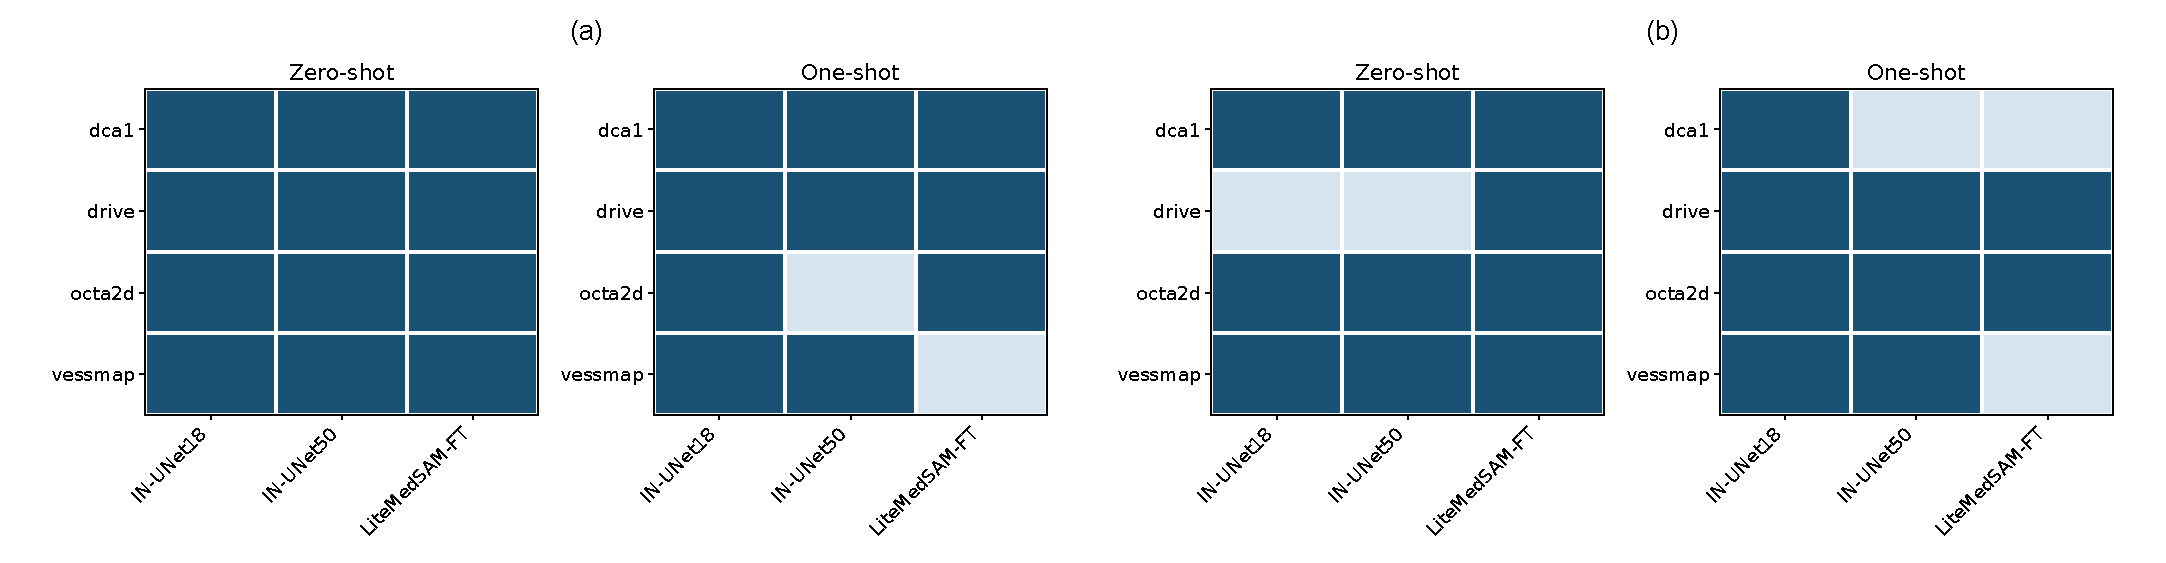
\includegraphics[width=\textwidth]{figures/dice_significance_analysis.pdf}
    \caption{Statistical-significance analysis of the Dice advantage of the VessShape-pretrained models over the baselines, using a one-sided paired Wilcoxon signed-rank test on per-image scores ($\alpha{=}0.05$, alternative ``greater''). (a) reference model VSUNet18; (b) reference model VSUNet50. Within each panel, the left grid is the zero-shot regime and the right grid the one-shot regime. Rows are datasets (DCA1, DRIVE, OCTA2D, VessMAP) and columns are the compared baselines (IN-UNet18, IN-UNet50, LiteMedSAM-FT). A dark cell indicates that the VSUNet reference is significantly better than that baseline on that dataset; a light cell indicates no significant difference.}
    \label{f:significance}
\end{figure*}


% #####################################################################
% # 5. TEXTO — Real-world data for validation
% #    DESTINO: substitui a subseção "Real-world data for validation" (l.224-235)
% #####################################################################
% >>> DESTINO: \subsection{Real-world data for validation}

To quantify the usefulness of the shape bias introduced by VessShape, we evaluate on four real-world blood vessel datasets that span three imaging modalities and very different visual characteristics: retinal fundus photography (DRIVE), retinal OCT angiography (OCTA2D), X-ray coronary angiography (DCA1), and fluorescence microscopy of the mouse cortex (VessMAP). Figure~\ref{f:drive_vessmap_samples} shows representative samples and ground-truth masks for each dataset.

The DRIVE dataset~\cite{Staal2004} is a popular standard for benchmarking retinal vessel segmentation, composed of 40 fundus photographs (20 training / 20 test), each measuring 584$\times$565 pixels. All DRIVE images were converted to grayscale prior to training, validation, and testing. The samples contain a clear global structure with landmarks such as the optic disk, and many very thin vessels that are challenging to segment.

The OCTA2D dataset is a 2D en-face retinal OCT-angiography collection derived from OCTA-500~\cite{Li2020_OCTA500}, in which the vasculature appears as a dense, high-contrast network of bright vessels on a dark background. Images were converted to grayscale and resized to 384$\times$384 pixels; the held-out test set contains 75 images.

The DCA1 dataset~\cite{Cervantes2019} consists of grayscale X-ray coronary angiograms (digital subtraction angiography). The vessels form a sparse, tree-like structure of coronary arteries over a low-contrast, non-uniform background, which makes this the most challenging domain in our study. Images were converted to grayscale and resized to 288$\times$288 pixels; the test set contains 21 images.

The VessMAP dataset~\cite{viana2025new} consists of 100 images, 256$\times$256 pixels each, acquired by fluorescence microscopy of the mouse cortex. It was curated to include challenging vascular characteristics, such as inconsistent noise and contrast levels, different vessel sizes, prominent imaging artifacts, and intensity fluctuations within vessel structures. Unlike DRIVE, the VessMAP images are highly magnified views with no discernible global organization and, without processing, contain bright vessels on a dark background.

Together, these datasets probe a broad range of textures, vessel densities, and calibers while sharing the same underlying tubular geometry, which is precisely the prior that VessShape aims to exploit.


% #####################################################################
% # 6. TEXTO — Model architectures and baselines
% #    DESTINO: substitui/expande "Model architectures and training strategies" (l.237-241)
% #####################################################################
% >>> DESTINO: \subsection{Model architectures and training strategies}

We adopt a U-Net architecture with a symmetrical encoder-decoder design and skip connections between corresponding stages. Two encoder capacities are considered, ResNet18 and ResNet50~\cite{he2016deep}, instantiated from the \textit{Segmentation Models PyTorch} package\footnote{\url{https://github.com/qubvel/segmentation_models.pytorch}}.

To isolate the effect of the shape bias, we compare four families of models that differ only in their initialization and training regime, keeping all other factors controlled:
\begin{itemize}
    \item \textbf{VSUNet18 / VSUNet50}: U-Nets whose weights are pre-trained on VessShape and then fine-tuned on the target dataset. These are our proposed models.
    \item \textbf{IN-UNet18 / IN-UNet50}: identical U-Nets whose encoders are initialized with ImageNet-pretrained weights and then fine-tuned. This is the standard transfer-learning baseline, which carries a texture-oriented prior rather than a shape prior.
    \item \textbf{LiteMedSAM-FT}: a lightweight variant of MedSAM (a Segment Anything model adapted to medical images)~\cite{ma2024medsam}, built on a TinyViT image encoder and a SAM-style mask decoder initialized with MedSAM weights. We fine-tune the image encoder and mask decoder (the prompt encoder is frozen and fed a fixed full-image box), so the model acts as a prompt-free semantic segmenter. This is a strong medical-foundation-model baseline.
    \item \textbf{U-Net18 / U-Net50}: the same U-Nets trained from scratch on the target dataset, providing a no-transfer reference.
\end{itemize}

The VSUNet-versus-IN-UNet comparison isolates the effect of a shape prior against a texture prior at matched capacity, while LiteMedSAM-FT contrasts our approach with a general-purpose medical foundation model. Table~\ref{tab:finetune_hparams} in the Appendix lists the per-dataset fine-tuning hyperparameters of the new baselines.


% #####################################################################
% # 7. TEXTO — nota sobre sequências N e cobertura scratch
% #    DESTINO: dentro de "Fine-tuning" (l.308) e "Training from scratch" (l.311-315)
% #####################################################################
% >>> DESTINO: parágrafo em \subsection{Fine-tuning}

In this work, we set $R=5$ and $S=3$. The sample-size sequence is $\mathcal{N}=\{1,2,4,6,8,10,12,14,16\}$ for DRIVE and $\mathcal{N}=\{1,2,4,6,8,10,12,14,16,18,20\}$ for OCTA2D, DCA1 and VessMAP. We also consider the zero-shot case ($n=0$), in which the pre-trained model is evaluated directly on $\mathcal{V}_{\text{test}}$ without any adaptation. Figure~\ref{f:training_protocol} summarizes the protocol.

% >>> DESTINO: nota de honestidade em \subsection{Training from scratch on real-world datasets}
% (opcional) Note that the from-scratch U-Net baselines could not be evaluated in every
% regime: DRIVE has no from-scratch run at the full-sample regime, and DCA1 has none at
% $n=1$. The corresponding cells are left empty in Tables~\ref{tab:combined_fewshot_percent}
% and~\ref{tab:full_metrics_appendix}.


% #####################################################################
% # 8. TEXTO — Results (reescrita enxuta em torno de 4 datasets + baselines)
% #    DESTINO: parte inicial de \section{Results} (l.318-393); manter os
% #    parágrafos qualitativos existentes (dip do VessMAP, CLIP etc.) que
% #    seguem válidos.
% #####################################################################

We report the Dice score as our main metric, as it is widely used in medical segmentation. Table~\ref{tab:combined_fewshot_percent} summarizes the zero-shot, one-shot and full-sample Dice for all models on the four datasets, and the complete set of metrics is given in Table~\ref{tab:full_metrics_appendix} (Appendix). Figure~\ref{f:results_charts} shows the full few-shot curves, and Figures~\ref{f:bar_zero_one} and~\ref{f:significance} focus on the extreme low-data regimes.

The most striking result is the \emph{zero-shot} behavior (Fig.~\ref{f:bar_zero_one}a). Only the VessShape-pretrained models transfer without any target training: VSUNet18 reaches a Dice of 76.6 on VessMAP, 55.3 on DRIVE and 53.6 on DCA1, and VSUNet50 reaches 47.0 on the difficult OCTA2D domain. In sharp contrast, both the ImageNet-pretrained IN-UNet and the MedSAM-initialized LiteMedSAM essentially fail in zero-shot (Dice near or below 20, and $\approx$0 for LiteMedSAM on all datasets). This confirms that a texture-oriented prior, however large the pre-training corpus, does not by itself localize vessels, whereas the VessShape shape prior does.

In the \emph{one-shot} regime (Fig.~\ref{f:bar_zero_one}b), a single labeled image is enough for every model to produce meaningful masks, and the VSUNet variants remain on top on DRIVE, VessMAP and DCA1 (VSUNet18 leading), while VSUNet50 marginally leads on OCTA2D. The Wilcoxon analysis (Fig.~\ref{f:significance}) shows that these one-shot advantages of VSUNet over the baselines are statistically significant on most dataset/baseline combinations, and even more so in zero-shot.

As the number of samples grows, the gap narrows and the ranking becomes dataset-dependent (Fig.~\ref{f:results_charts}). At the full-sample regime, VSUNet remains competitive everywhere and best on some domains (VSUNet18 attains 87.1 on OCTA2D and VSUNet50 79.9 on DRIVE), while the fine-tuned LiteMedSAM-FT, given enough data, achieves the best full-shot Dice on VessMAP (89.5) and DCA1 (76.9). On OCTA2D---an easy, high-contrast domain---all models converge to a similar Dice. Overall, the pre-trained VSUNet models consistently rise faster and exhibit lower variance in the few-shot regime, and retain an advantage over the from-scratch U-Nets even with all samples available, indicating that the shape bias remains beneficial as data increases.


% #####################################################################
% # 9. TABELA (CORPO) — compact Dice, substitui tab:combined_fewshot_percent
% #####################################################################
\begin{table*}[t]
    \caption{Dice score (\%) for zero-shot ($n{=}0$), one-shot ($n{=}1$) and full-sample ($n{=}16$ for DRIVE, $n{=}20$ otherwise) segmentation on the four datasets. Values are mean $\pm$ standard deviation over repeated runs ($R{=}5$, $S{=}3$); zero-shot rows come from a single inference and thus have zero deviation. For $n{=}0$, the LiteMedSAM-FT column reports the un-fine-tuned LiteMedSAM. Best value per row in \textbf{bold}; ``---'' marks configurations that were not evaluated.}
    \label{tab:combined_fewshot_percent}
    \centering
    \begingroup
    \small
    \setlength{\tabcolsep}{4pt}
    \renewcommand{\arraystretch}{1.15}
\begin{tabular}{l r r r r r r r r }
\hline
\textbf{Dataset} & \textbf{N} & \textbf{VSUNet18} & \textbf{VSUNet50} & \textbf{IN-UNet18} & \textbf{IN-UNet50} & \textbf{LiteMedSAM-FT} & \textbf{UNet18} & \textbf{UNet50} \\
\hline
\multirow{3}{*}{DRIVE} & 0 & $\mathbf{55.3} \,\pm\, 0.0$ & $17.5 \,\pm\, 0.0$ & $17.2 \,\pm\, 0.0$ & $22.6 \,\pm\, 0.0$ & $0.0 \,\pm\, 0.0$ & --- & --- \\
 & 1 & $\mathbf{76.1} \,\pm\, 0.7$ & $75.3 \,\pm\, 1.5$ & $72.0 \,\pm\, 3.5$ & $73.5 \,\pm\, 2.7$ & $66.5 \,\pm\, 7.5$ & $65.8 \,\pm\, 9.5$ & $68.4 \,\pm\, 4.6$ \\
 & 16 & $79.7 \,\pm\, 0.1$ & $\mathbf{79.9} \,\pm\, 0.1$ & $79.4 \,\pm\, 0.3$ & $79.2 \,\pm\, 0.1$ & $78.4 \,\pm\, 0.2$ & --- & --- \\
\hline
\multirow{3}{*}{OCTA2D} & 0 & $27.2 \,\pm\, 0.0$ & $\mathbf{47.0} \,\pm\, 0.0$ & $13.8 \,\pm\, 0.0$ & $15.1 \,\pm\, 0.0$ & $0.0 \,\pm\, 0.0$ & --- & --- \\
 & 1 & $80.4 \,\pm\, 2.1$ & $\mathbf{80.5} \,\pm\, 2.1$ & $80.0 \,\pm\, 2.2$ & $80.2 \,\pm\, 3.0$ & $78.7 \,\pm\, 4.1$ & $78.0 \,\pm\, 4.2$ & $79.6 \,\pm\, 2.6$ \\
 & 20 & $\mathbf{87.1} \,\pm\, 0.3$ & $85.7 \,\pm\, 0.2$ & $86.5 \,\pm\, 0.2$ & $85.9 \,\pm\, 0.2$ & $86.2 \,\pm\, 0.4$ & $87.0 \,\pm\, 0.6$ & $86.4 \,\pm\, 0.3$ \\
\hline
\multirow{3}{*}{DCA1} & 0 & $\mathbf{53.6} \,\pm\, 0.0$ & $48.0 \,\pm\, 0.0$ & $5.5 \,\pm\, 0.0$ & $9.2 \,\pm\, 0.0$ & $0.9 \,\pm\, 0.0$ & --- & --- \\
 & 1 & $\mathbf{54.7} \,\pm\, 7.9$ & $46.8 \,\pm\, 12.3$ & $30.5 \,\pm\, 16.1$ & $45.6 \,\pm\, 12.3$ & $50.9 \,\pm\, 12.1$ & --- & --- \\
 & 20 & $76.7 \,\pm\, 1.3$ & $75.6 \,\pm\, 1.7$ & $72.6 \,\pm\, 2.8$ & $75.7 \,\pm\, 1.4$ & $\mathbf{76.9} \,\pm\, 0.7$ & $71.2 \,\pm\, 2.3$ & $71.9 \,\pm\, 2.8$ \\
\hline
\multirow{3}{*}{VessMAP} & 0 & $\mathbf{76.6} \,\pm\, 0.0$ & $63.8 \,\pm\, 0.0$ & $10.3 \,\pm\, 0.0$ & $36.6 \,\pm\, 0.0$ & $0.0 \,\pm\, 0.0$ & --- & --- \\
 & 1 & $\mathbf{59.7} \,\pm\, 12.4$ & $58.4 \,\pm\, 11.4$ & $48.6 \,\pm\, 8.2$ & $53.4 \,\pm\, 8.7$ & $58.1 \,\pm\, 11.7$ & $49.1 \,\pm\, 6.0$ & $48.0 \,\pm\, 6.5$ \\
 & 20 & $85.7 \,\pm\, 1.5$ & $84.3 \,\pm\, 1.4$ & $82.2 \,\pm\, 2.9$ & $84.2 \,\pm\, 1.4$ & $\mathbf{89.5} \,\pm\, 0.6$ & $83.0 \,\pm\, 2.4$ & $72.6 \,\pm\, 4.4$ \\
\hline
\end{tabular}
    \endgroup
\end{table*}


% #####################################################################
% # 10. TABELA (APÊNDICE) — full 5-metric
% #####################################################################
\begin{table*}[t]
    \caption{Complete segmentation metrics (\%) for zero-shot, one-shot and full-sample regimes on the four datasets. Values are mean $\pm$ standard deviation over repeated runs; zero-shot rows come from a single inference. Best Dice per (dataset, $N$) group in \textbf{bold}.}
    \label{tab:full_metrics_appendix}
    \centering
    \begingroup
    \footnotesize
    \setlength{\tabcolsep}{3pt}
    \renewcommand{\arraystretch}{1.12}
\begin{tabular}{l c l r r r r r r}
\hline
\textbf{Dataset} & \textbf{N} & \textbf{Model} & \textbf{Dice} & \textbf{Acc} & \textbf{IoU} & \textbf{Prec} & \textbf{Rec} & \textbf{AUC} \\
\hline
\multirow{17}{*}{DRIVE} & \multirow{5}{*}{0} & VSUNet18 & $\mathbf{55.3} \,\pm\, 0.0$ & $88.9 \,\pm\, 0.0$ & $38.9 \,\pm\, 0.0$ & $59.4 \,\pm\, 0.0$ & $57.7 \,\pm\, 0.0$ & $85.5 \,\pm\, 0.0$ \\
 &  & VSUNet50 & $17.5 \,\pm\, 0.0$ & $88.1 \,\pm\, 0.0$ & $10.1 \,\pm\, 0.0$ & $72.1 \,\pm\, 0.0$ & $11.0 \,\pm\, 0.0$ & $71.6 \,\pm\, 0.0$ \\
 &  & IN-UNet18 & $17.2 \,\pm\, 0.0$ & $52.8 \,\pm\, 0.0$ & $9.4 \,\pm\, 0.0$ & $11.1 \,\pm\, 0.0$ & $38.8 \,\pm\, 0.0$ & $44.6 \,\pm\, 0.0$ \\
 &  & IN-UNet50 & $22.6 \,\pm\, 0.0$ & $12.7 \,\pm\, 0.0$ & $12.7 \,\pm\, 0.0$ & $12.7 \,\pm\, 0.0$ & $100.0 \,\pm\, 0.0$ & $49.8 \,\pm\, 0.0$ \\
 &  & LiteMedSAM-FT & $0.0 \,\pm\, 0.0$ & $87.3 \,\pm\, 0.0$ & $0.0 \,\pm\, 0.0$ & $0.0 \,\pm\, 0.0$ & $0.0 \,\pm\, 0.0$ & $51.0 \,\pm\, 0.0$ \\
\cline{2-9}
 & \multirow{7}{*}{1} & VSUNet18 & $\mathbf{76.1} \,\pm\, 0.7$ & $94.1 \,\pm\, 0.3$ & $61.5 \,\pm\, 0.9$ & $78.2 \,\pm\, 2.3$ & $74.9 \,\pm\, 1.9$ & $94.8 \,\pm\, 0.5$ \\
 &  & VSUNet50 & $75.3 \,\pm\, 1.5$ & $93.8 \,\pm\, 0.7$ & $60.5 \,\pm\, 1.9$ & $76.7 \,\pm\, 4.8$ & $75.1 \,\pm\, 4.3$ & $94.8 \,\pm\, 0.5$ \\
 &  & IN-UNet18 & $72.0 \,\pm\, 3.5$ & $92.5 \,\pm\, 1.9$ & $56.6 \,\pm\, 4.1$ & $72.7 \,\pm\, 8.9$ & $74.9 \,\pm\, 9.3$ & $94.4 \,\pm\, 1.2$ \\
 &  & IN-UNet50 & $73.5 \,\pm\, 2.7$ & $93.3 \,\pm\, 0.7$ & $58.2 \,\pm\, 3.2$ & $75.1 \,\pm\, 7.2$ & $74.3 \,\pm\, 9.0$ & $95.0 \,\pm\, 0.7$ \\
 &  & LiteMedSAM-FT & $66.5 \,\pm\, 7.5$ & $92.7 \,\pm\, 0.9$ & $51.0 \,\pm\, 7.6$ & $78.8 \,\pm\, 4.6$ & $60.4 \,\pm\, 10.6$ & $91.3 \,\pm\, 4.4$ \\
 &  & UNet18 & $65.8 \,\pm\, 9.5$ & $91.0 \,\pm\, 3.4$ & $50.0 \,\pm\, 9.5$ & $71.1 \,\pm\, 10.7$ & $67.2 \,\pm\, 14.8$ & $92.0 \,\pm\, 3.2$ \\
 &  & UNet50 & $68.4 \,\pm\, 4.6$ & $92.3 \,\pm\, 0.9$ & $52.5 \,\pm\, 4.9$ & $73.3 \,\pm\, 7.4$ & $67.5 \,\pm\, 10.5$ & $91.6 \,\pm\, 2.2$ \\
\cline{2-9}
 & \multirow{5}{*}{16} & VSUNet18 & $79.7 \,\pm\, 0.1$ & $95.0 \,\pm\, 0.0$ & $66.3 \,\pm\, 0.1$ & $82.9 \,\pm\, 0.3$ & $77.2 \,\pm\, 0.3$ & $96.7 \,\pm\, 0.0$ \\
 &  & VSUNet50 & $\mathbf{79.9} \,\pm\, 0.1$ & $95.1 \,\pm\, 0.0$ & $66.6 \,\pm\, 0.1$ & $84.1 \,\pm\, 0.2$ & $76.6 \,\pm\, 0.2$ & $96.9 \,\pm\, 0.0$ \\
 &  & IN-UNet18 & $79.4 \,\pm\, 0.3$ & $94.9 \,\pm\, 0.1$ & $65.9 \,\pm\, 0.4$ & $81.3 \,\pm\, 0.7$ & $78.1 \,\pm\, 0.6$ & $96.7 \,\pm\, 0.1$ \\
 &  & IN-UNet50 & $79.2 \,\pm\, 0.1$ & $94.8 \,\pm\, 0.0$ & $65.6 \,\pm\, 0.1$ & $80.4 \,\pm\, 0.4$ & $78.6 \,\pm\, 0.5$ & $96.5 \,\pm\, 0.0$ \\
 &  & LiteMedSAM-FT & $78.4 \,\pm\, 0.2$ & $94.9 \,\pm\, 0.0$ & $64.5 \,\pm\, 0.3$ & $85.0 \,\pm\, 0.4$ & $73.3 \,\pm\, 0.5$ & $96.9 \,\pm\, 0.1$ \\
\hline
\multirow{19}{*}{OCTA2D} & \multirow{5}{*}{0} & VSUNet18 & $27.2 \,\pm\, 0.0$ & $90.7 \,\pm\, 0.0$ & $17.9 \,\pm\, 0.0$ & $70.4 \,\pm\, 0.0$ & $35.1 \,\pm\, 0.0$ & $78.2 \,\pm\, 0.0$ \\
 &  & VSUNet50 & $\mathbf{47.0} \,\pm\, 0.0$ & $92.3 \,\pm\, 0.0$ & $31.9 \,\pm\, 0.0$ & $71.4 \,\pm\, 0.0$ & $45.1 \,\pm\, 0.0$ & $84.6 \,\pm\, 0.0$ \\
 &  & IN-UNet18 & $13.8 \,\pm\, 0.0$ & $86.3 \,\pm\, 0.0$ & $7.5 \,\pm\, 0.0$ & $15.3 \,\pm\, 0.0$ & $14.2 \,\pm\, 0.0$ & $58.7 \,\pm\, 0.0$ \\
 &  & IN-UNet50 & $15.1 \,\pm\, 0.0$ & $9.1 \,\pm\, 0.0$ & $8.2 \,\pm\, 0.0$ & $8.2 \,\pm\, 0.0$ & $98.9 \,\pm\, 0.0$ & $44.8 \,\pm\, 0.0$ \\
 &  & LiteMedSAM-FT & $0.0 \,\pm\, 0.0$ & $91.8 \,\pm\, 0.0$ & $0.0 \,\pm\, 0.0$ & $0.0 \,\pm\, 0.0$ & $0.0 \,\pm\, 0.0$ & $61.3 \,\pm\, 0.0$ \\
\cline{2-9}
 & \multirow{7}{*}{1} & VSUNet18 & $80.4 \,\pm\, 2.1$ & $96.8 \,\pm\, 0.5$ & $67.8 \,\pm\, 2.6$ & $84.3 \,\pm\, 7.4$ & $80.0 \,\pm\, 8.0$ & $98.1 \,\pm\, 0.9$ \\
 &  & VSUNet50 & $\mathbf{80.5} \,\pm\, 2.1$ & $97.0 \,\pm\, 0.2$ & $67.8 \,\pm\, 2.8$ & $86.0 \,\pm\, 5.8$ & $77.6 \,\pm\, 7.3$ & $97.9 \,\pm\, 1.2$ \\
 &  & IN-UNet18 & $80.0 \,\pm\, 2.2$ & $96.9 \,\pm\, 0.3$ & $67.2 \,\pm\, 2.9$ & $85.3 \,\pm\, 6.9$ & $77.9 \,\pm\, 7.8$ & $97.7 \,\pm\, 1.1$ \\
 &  & IN-UNet50 & $80.2 \,\pm\, 3.0$ & $96.9 \,\pm\, 0.3$ & $67.5 \,\pm\, 3.7$ & $85.4 \,\pm\, 6.4$ & $78.1 \,\pm\, 8.8$ & $97.7 \,\pm\, 1.6$ \\
 &  & LiteMedSAM-FT & $78.7 \,\pm\, 4.1$ & $96.8 \,\pm\, 0.3$ & $65.6 \,\pm\, 4.9$ & $85.8 \,\pm\, 6.0$ & $75.6 \,\pm\, 10.1$ & $97.7 \,\pm\, 1.3$ \\
 &  & UNet18 & $78.0 \,\pm\, 4.2$ & $96.7 \,\pm\, 0.4$ & $64.8 \,\pm\, 4.9$ & $85.1 \,\pm\, 6.6$ & $75.1 \,\pm\, 10.1$ & $96.4 \,\pm\, 2.8$ \\
 &  & UNet50 & $79.6 \,\pm\, 2.6$ & $96.9 \,\pm\, 0.2$ & $66.7 \,\pm\, 3.3$ & $85.7 \,\pm\, 5.8$ & $76.8 \,\pm\, 8.4$ & $97.0 \,\pm\, 2.1$ \\
\cline{2-9}
 & \multirow{7}{*}{20} & VSUNet18 & $\mathbf{87.1} \,\pm\, 0.3$ & $97.9 \,\pm\, 0.1$ & $77.3 \,\pm\, 0.5$ & $89.6 \,\pm\, 0.9$ & $85.0 \,\pm\, 0.7$ & $99.3 \,\pm\, 0.0$ \\
 &  & VSUNet50 & $85.7 \,\pm\, 0.2$ & $97.7 \,\pm\, 0.0$ & $75.1 \,\pm\, 0.3$ & $88.0 \,\pm\, 0.7$ & $83.7 \,\pm\, 1.0$ & $99.2 \,\pm\, 0.0$ \\
 &  & IN-UNet18 & $86.5 \,\pm\, 0.2$ & $97.8 \,\pm\, 0.1$ & $76.4 \,\pm\, 0.4$ & $88.6 \,\pm\, 1.0$ & $84.7 \,\pm\, 0.6$ & $99.3 \,\pm\, 0.0$ \\
 &  & IN-UNet50 & $85.9 \,\pm\, 0.2$ & $97.7 \,\pm\, 0.0$ & $75.4 \,\pm\, 0.2$ & $88.3 \,\pm\, 0.8$ & $83.8 \,\pm\, 0.8$ & $99.1 \,\pm\, 0.0$ \\
 &  & LiteMedSAM-FT & $86.2 \,\pm\, 0.4$ & $97.8 \,\pm\, 0.1$ & $75.8 \,\pm\, 0.6$ & $90.1 \,\pm\, 0.5$ & $82.8 \,\pm\, 0.9$ & $99.1 \,\pm\, 0.1$ \\
 &  & UNet18 & $87.0 \,\pm\, 0.6$ & $97.9 \,\pm\, 0.1$ & $77.1 \,\pm\, 0.9$ & $89.0 \,\pm\, 1.1$ & $85.3 \,\pm\, 0.8$ & $99.3 \,\pm\, 0.1$ \\
 &  & UNet50 & $86.4 \,\pm\, 0.3$ & $97.8 \,\pm\, 0.1$ & $76.2 \,\pm\, 0.4$ & $88.7 \,\pm\, 0.9$ & $84.4 \,\pm\, 0.7$ & $99.2 \,\pm\, 0.0$ \\
\hline
\multirow{17}{*}{DCA1} & \multirow{5}{*}{0} & VSUNet18 & $\mathbf{53.6} \,\pm\, 0.0$ & $91.3 \,\pm\, 0.0$ & $37.5 \,\pm\, 0.0$ & $40.1 \,\pm\, 0.0$ & $91.7 \,\pm\, 0.0$ & $97.1 \,\pm\, 0.0$ \\
 &  & VSUNet50 & $48.0 \,\pm\, 0.0$ & $92.9 \,\pm\, 0.0$ & $33.2 \,\pm\, 0.0$ & $42.7 \,\pm\, 0.0$ & $70.7 \,\pm\, 0.0$ & $92.6 \,\pm\, 0.0$ \\
 &  & IN-UNet18 & $5.5 \,\pm\, 0.0$ & $79.6 \,\pm\, 0.0$ & $2.9 \,\pm\, 0.0$ & $3.7 \,\pm\, 0.0$ & $13.1 \,\pm\, 0.0$ & $40.5 \,\pm\, 0.0$ \\
 &  & IN-UNet50 & $9.2 \,\pm\, 0.0$ & $6.2 \,\pm\, 0.0$ & $4.8 \,\pm\, 0.0$ & $4.8 \,\pm\, 0.0$ & $99.8 \,\pm\, 0.0$ & $54.6 \,\pm\, 0.0$ \\
 &  & LiteMedSAM-FT & $0.9 \,\pm\, 0.0$ & $95.2 \,\pm\, 0.0$ & $0.5 \,\pm\, 0.0$ & $17.0 \,\pm\, 0.0$ & $0.5 \,\pm\, 0.0$ & $69.6 \,\pm\, 0.0$ \\
\cline{2-9}
 & \multirow{5}{*}{1} & VSUNet18 & $\mathbf{54.7} \,\pm\, 7.9$ & $96.7 \,\pm\, 0.5$ & $40.4 \,\pm\, 7.3$ & $75.2 \,\pm\, 7.7$ & $49.0 \,\pm\, 12.7$ & $92.5 \,\pm\, 4.3$ \\
 &  & VSUNet50 & $46.8 \,\pm\, 12.3$ & $96.5 \,\pm\, 0.3$ & $33.2 \,\pm\, 10.5$ & $77.6 \,\pm\, 8.1$ & $39.6 \,\pm\, 16.1$ & $89.3 \,\pm\, 5.1$ \\
 &  & IN-UNet18 & $30.5 \,\pm\, 16.1$ & $95.1 \,\pm\, 2.3$ & $20.3 \,\pm\, 12.5$ & $64.1 \,\pm\, 20.2$ & $27.2 \,\pm\, 17.3$ & $78.1 \,\pm\, 13.0$ \\
 &  & IN-UNet50 & $45.6 \,\pm\, 12.3$ & $96.3 \,\pm\, 0.4$ & $31.9 \,\pm\, 10.5$ & $75.5 \,\pm\, 10.4$ & $39.0 \,\pm\, 16.6$ & $85.4 \,\pm\, 6.0$ \\
 &  & LiteMedSAM-FT & $50.9 \,\pm\, 12.1$ & $95.1 \,\pm\, 4.0$ & $36.5 \,\pm\, 10.8$ & $69.4 \,\pm\, 21.1$ & $48.8 \,\pm\, 12.7$ & $91.9 \,\pm\, 5.1$ \\
\cline{2-9}
 & \multirow{7}{*}{20} & VSUNet18 & $76.7 \,\pm\, 1.3$ & $97.8 \,\pm\, 0.1$ & $62.6 \,\pm\, 1.6$ & $79.0 \,\pm\, 1.4$ & $76.0 \,\pm\, 2.9$ & $99.0 \,\pm\, 0.1$ \\
 &  & VSUNet50 & $75.6 \,\pm\, 1.7$ & $97.7 \,\pm\, 0.1$ & $61.3 \,\pm\, 1.9$ & $78.1 \,\pm\, 1.4$ & $75.1 \,\pm\, 3.4$ & $98.6 \,\pm\, 0.2$ \\
 &  & IN-UNet18 & $72.6 \,\pm\, 2.8$ & $97.5 \,\pm\, 0.1$ & $57.9 \,\pm\, 2.8$ & $77.2 \,\pm\, 2.4$ & $71.7 \,\pm\, 4.8$ & $98.4 \,\pm\, 0.3$ \\
 &  & IN-UNet50 & $75.7 \,\pm\, 1.4$ & $97.8 \,\pm\, 0.1$ & $61.3 \,\pm\, 1.7$ & $78.5 \,\pm\, 1.2$ & $74.6 \,\pm\, 3.0$ & $97.9 \,\pm\, 0.4$ \\
 &  & LiteMedSAM-FT & $\mathbf{76.9} \,\pm\, 0.7$ & $97.8 \,\pm\, 0.0$ & $62.8 \,\pm\, 0.9$ & $77.3 \,\pm\, 1.1$ & $78.1 \,\pm\, 1.7$ & $98.7 \,\pm\, 0.2$ \\
 &  & UNet18 & $71.2 \,\pm\, 2.3$ & $97.4 \,\pm\, 0.2$ & $56.2 \,\pm\, 2.1$ & $75.7 \,\pm\, 3.7$ & $70.8 \,\pm\, 5.2$ & $98.2 \,\pm\, 0.3$ \\
 &  & UNet50 & $71.9 \,\pm\, 2.8$ & $97.5 \,\pm\, 0.1$ & $57.2 \,\pm\, 2.7$ & $76.8 \,\pm\, 2.3$ & $71.0 \,\pm\, 5.0$ & $97.9 \,\pm\, 0.6$ \\
\hline
\multirow{19}{*}{VessMAP} & \multirow{5}{*}{0} & VSUNet18 & $\mathbf{76.6} \,\pm\, 0.0$ & $90.7 \,\pm\, 0.0$ & $62.9 \,\pm\, 0.0$ & $86.1 \,\pm\, 0.0$ & $70.8 \,\pm\, 0.0$ & $94.8 \,\pm\, 0.0$ \\
 &  & VSUNet50 & $63.8 \,\pm\, 0.0$ & $84.9 \,\pm\, 0.0$ & $49.7 \,\pm\, 0.0$ & $73.5 \,\pm\, 0.0$ & $61.8 \,\pm\, 0.0$ & $88.3 \,\pm\, 0.0$ \\
 &  & IN-UNet18 & $10.3 \,\pm\, 0.0$ & $72.7 \,\pm\, 0.0$ & $5.5 \,\pm\, 0.0$ & $23.1 \,\pm\, 0.0$ & $7.8 \,\pm\, 0.0$ & $46.3 \,\pm\, 0.0$ \\
 &  & IN-UNet50 & $36.6 \,\pm\, 0.0$ & $23.8 \,\pm\, 0.0$ & $22.9 \,\pm\, 0.0$ & $23.0 \,\pm\, 0.0$ & $98.7 \,\pm\, 0.0$ & $56.3 \,\pm\, 0.0$ \\
 &  & LiteMedSAM-FT & $0.0 \,\pm\, 0.0$ & $77.1 \,\pm\, 0.0$ & $0.0 \,\pm\, 0.0$ & $0.0 \,\pm\, 0.0$ & $0.0 \,\pm\, 0.0$ & $59.5 \,\pm\, 0.0$ \\
\cline{2-9}
 & \multirow{7}{*}{1} & VSUNet18 & $\mathbf{59.7} \,\pm\, 12.4$ & $69.5 \,\pm\, 24.6$ & $46.6 \,\pm\, 12.8$ & $61.7 \,\pm\, 22.5$ & $78.5 \,\pm\, 12.8$ & $85.9 \,\pm\, 12.6$ \\
 &  & VSUNet50 & $58.4 \,\pm\, 11.4$ & $69.2 \,\pm\, 24.3$ & $45.4 \,\pm\, 11.8$ & $63.2 \,\pm\, 22.8$ & $76.1 \,\pm\, 14.8$ & $85.1 \,\pm\, 11.1$ \\
 &  & IN-UNet18 & $48.6 \,\pm\, 8.2$ & $65.1 \,\pm\, 15.5$ & $35.8 \,\pm\, 7.9$ & $58.6 \,\pm\, 18.7$ & $66.1 \,\pm\, 18.0$ & $78.1 \,\pm\, 8.7$ \\
 &  & IN-UNet50 & $53.4 \,\pm\, 8.7$ & $66.7 \,\pm\, 22.4$ & $40.3 \,\pm\, 9.0$ & $62.7 \,\pm\, 22.5$ & $71.2 \,\pm\, 16.9$ & $84.1 \,\pm\, 3.9$ \\
 &  & LiteMedSAM-FT & $58.1 \,\pm\, 11.7$ & $75.5 \,\pm\, 21.3$ & $45.9 \,\pm\, 12.6$ & $69.1 \,\pm\, 21.4$ & $67.2 \,\pm\, 16.8$ & $83.3 \,\pm\, 13.2$ \\
 &  & UNet18 & $49.1 \,\pm\, 6.0$ & $63.3 \,\pm\, 19.9$ & $36.2 \,\pm\, 6.3$ & $59.2 \,\pm\, 19.1$ & $70.2 \,\pm\, 16.6$ & $80.4 \,\pm\, 9.6$ \\
 &  & UNet50 & $48.0 \,\pm\, 6.5$ & $59.4 \,\pm\, 21.6$ & $34.8 \,\pm\, 6.8$ & $55.4 \,\pm\, 20.2$ & $72.8 \,\pm\, 17.6$ & $78.2 \,\pm\, 7.8$ \\
\cline{2-9}
 & \multirow{7}{*}{20} & VSUNet18 & $85.7 \,\pm\, 1.5$ & $93.0 \,\pm\, 1.2$ & $76.2 \,\pm\, 2.0$ & $86.1 \,\pm\, 4.1$ & $87.3 \,\pm\, 5.2$ & $97.3 \,\pm\, 0.3$ \\
 &  & VSUNet50 & $84.3 \,\pm\, 1.4$ & $92.8 \,\pm\, 1.2$ & $74.0 \,\pm\, 1.8$ & $87.6 \,\pm\, 2.7$ & $83.3 \,\pm\, 2.8$ & $96.9 \,\pm\, 0.6$ \\
 &  & IN-UNet18 & $82.2 \,\pm\, 2.9$ & $92.3 \,\pm\, 1.0$ & $71.3 \,\pm\, 3.7$ & $86.3 \,\pm\, 3.0$ & $81.1 \,\pm\, 6.1$ & $96.5 \,\pm\, 0.5$ \\
 &  & IN-UNet50 & $84.2 \,\pm\, 1.4$ & $93.2 \,\pm\, 0.9$ & $74.1 \,\pm\, 1.7$ & $88.4 \,\pm\, 3.2$ & $82.1 \,\pm\, 3.9$ & $96.9 \,\pm\, 0.3$ \\
 &  & LiteMedSAM-FT & $\mathbf{89.5} \,\pm\, 0.6$ & $95.3 \,\pm\, 0.3$ & $81.8 \,\pm\, 0.8$ & $88.5 \,\pm\, 1.9$ & $91.8 \,\pm\, 1.4$ & $98.6 \,\pm\, 0.2$ \\
 &  & UNet18 & $83.0 \,\pm\, 2.4$ & $91.6 \,\pm\, 1.1$ & $72.0 \,\pm\, 2.9$ & $81.3 \,\pm\, 2.7$ & $87.0 \,\pm\, 6.0$ & $97.0 \,\pm\, 0.5$ \\
 &  & UNet50 & $72.6 \,\pm\, 4.4$ & $87.9 \,\pm\, 2.0$ & $59.5 \,\pm\, 5.1$ & $84.3 \,\pm\, 3.9$ & $70.1 \,\pm\, 6.9$ & $92.6 \,\pm\, 1.7$ \\
\hline
\end{tabular}
    \endgroup
\end{table*}


% #####################################################################
% # 11. TABELA (APÊNDICE) — hiperparâmetros de fine-tuning dos baselines
% #####################################################################
\begin{table}[t]
    \caption{Per-dataset fine-tuning setup for the baseline models. Input side is the resize used for the U-Net variants; LiteMedSAM-FT always uses RGB 256$\times$256. All runs use the Adam optimizer, up to 500 epochs, and last-checkpoint selection.}
    \label{tab:finetune_hparams}
    \centering
    \begingroup
    \small
    \setlength{\tabcolsep}{5pt}
    \renewcommand{\arraystretch}{1.15}
    \begin{tabular}{l l l l}
        \hline
        \textbf{Model} & \textbf{Input} & \textbf{Loss} & \textbf{LR} \\
        \hline
        IN-UNet18 / VSUNet18 & gray, per-dataset$^{\dagger}$ & cross-entropy & $10^{-2}$ \\
        IN-UNet50 / VSUNet50 & gray, per-dataset$^{\dagger}$ & cross-entropy & $10^{-3}$ \\
        LiteMedSAM-FT & RGB, $256{\times}256$ & BCE & $10^{-3}$ \\
        \hline
    \end{tabular}
    \endgroup
    \\[2pt]
    {\footnotesize $^{\dagger}$ Resize: DRIVE $512{\times}512$, OCTA2D $384{\times}384$, DCA1 $288{\times}288$, VessMAP $256{\times}256$.}
\end{table}


% #####################################################################
% # 12. CONCLUSÃO — trecho a mesclar em \section{Conclusion} (l.398-409)
% #####################################################################
% >>> DESTINO: substituir a frase "two distinct and challenging real-world datasets, DRIVE ... and VessMAP ..."
Our experiments demonstrated the effectiveness of this approach across four datasets spanning three imaging modalities: retinal fundus photography (DRIVE), retinal OCT angiography (OCTA2D), X-ray coronary angiography (DCA1), and cerebral cortex microscopy (VessMAP). A model pre-trained on VessShape achieved strong few-shot performance on all of them and, crucially, was the only strategy to exhibit non-trivial \emph{zero-shot} segmentation: standard ImageNet-pretrained U-Nets and a fine-tuned medical foundation model (LiteMedSAM) failed without any target supervision, whereas the shape-biased VSUNet segmented vessels directly. These results confirm our hypothesis that leveraging a geometric prior is an effective strategy to improve data efficiency and robustness against domain shifts.


\end{document}
